\documentclass[times, utf8, seminar]{fer}
\usepackage{booktabs}
\usepackage{graphicx}
\usepackage{float}
\usepackage{algorithm}
\usepackage{algorithmic}

\begin{document}

% TODO: Navedite naslov rada.
\title{Poboljšanje djelomično sastavljenog genoma dugim očitanjima}

% TODO: Navedite vaše ime i prezime.
\author{Lana Tuković, Ema Vlainić}

% TODO: Navedite ime i prezime mentora.
\voditelj{Krešimir Križanović}

\maketitle

\tableofcontents

\chapter{Uvod}
Postupak sastavljanja složenih genoma može dati fragmentiran rezultat zbog velikog broja ponavljajućih sekvenci koje otežavaju proces poravnanja. Naš zadatak bio je pokušati međusobno povezati dobivene fragmente - contige u cijeli genom. Algoritam koji smo pri tome koristili zasniva se na konstruiranju grafa preklapanja te pronalaženja optimalnih staza među preklapanjima. Pronađena optimalna staza će nam služiti da povežemo dva contig-a.

\chapter{Opis algoritma}
Skupovi očitanja i već sastavljenih contig-a pripremljeni su kao testni podaci. Njihova preklapanja dobivena pomoću alata Minimap2 koristimo kao ulazne točke programa.

\underline{Ulazni podaci:}
\begin{itemize}
	\item[•]{preklapanja između contig-a i očitanja u PAF formatu dobivena korištenjem alata Minimap2 \cite{minimap2} nad datotekom sa skupom contig-a i datotekom sa skupom očitanja}
	\item[•]{međusobna preklapanja očitanja u PAF formatu dobivena korištenjem alata Minimap2 nad dvije iste datoteke sa skupom očitanja}
\end{itemize}

\underline{Izlazni podaci:}
\begin{itemize}
	\item[•]{poboljšani skup sastavljenih contiga u FASTA formatu}
\end{itemize}

\begin{flushleft}
Sada kada imamo sve potrebne podatke možemo konstruirati graf preklapanja. U svom radu \cite{du2021assembly} opisali su postupak kontruiranja grafa preklapanja gdje preklapanja povezuju čvorove grafa. Graf preklapanja sastoji se od dvije vrste čvorova: usidreni čvorovi (\textit{anchoring nodes}) koji predstavljaju unaprijed sastavljane contig-e i čvorovi očitanja (\textit{read nodes}). Veza između dva čvorova predstavlja preklapanje tih dvaju čvorova. Kada je graf konstruiran, slijedi traženje optimalnih staza iz svakog usidrenog čvora do skupa mogućih završnih usidrenih čvorova.

Postupak traženja staza provodi se tako da se iz svakog čvora širi staza prema susjednom čvoru sa najvećim dobitkom. Optimalne staze u grafu tražili smo na tri načina:
\begin{itemize}
	\item[•]{staza se proširuje na susjedni čvor koji ima najveći \textit{overlap score} - vrijednost preklapanja}
	\item[•]{staza se proširuje na susjedni čvor koji ima najveći \textit{extension score} - vrijednost nadovezivanja}
	\item[•]{staza se proširuje na susjedni čvor koji je slučajno izabran, a vjerovatnost njegovog izabiranja je proporcionalna njegovoj vrijednosti nadovezivanja - \textit{Monte Carlo} metoda}

Na slici \ref{fig:scores} prikazano je kako se računa \textit{overlap score} i \textit{extension score}.

\begin{figure}[H]
  \centering
  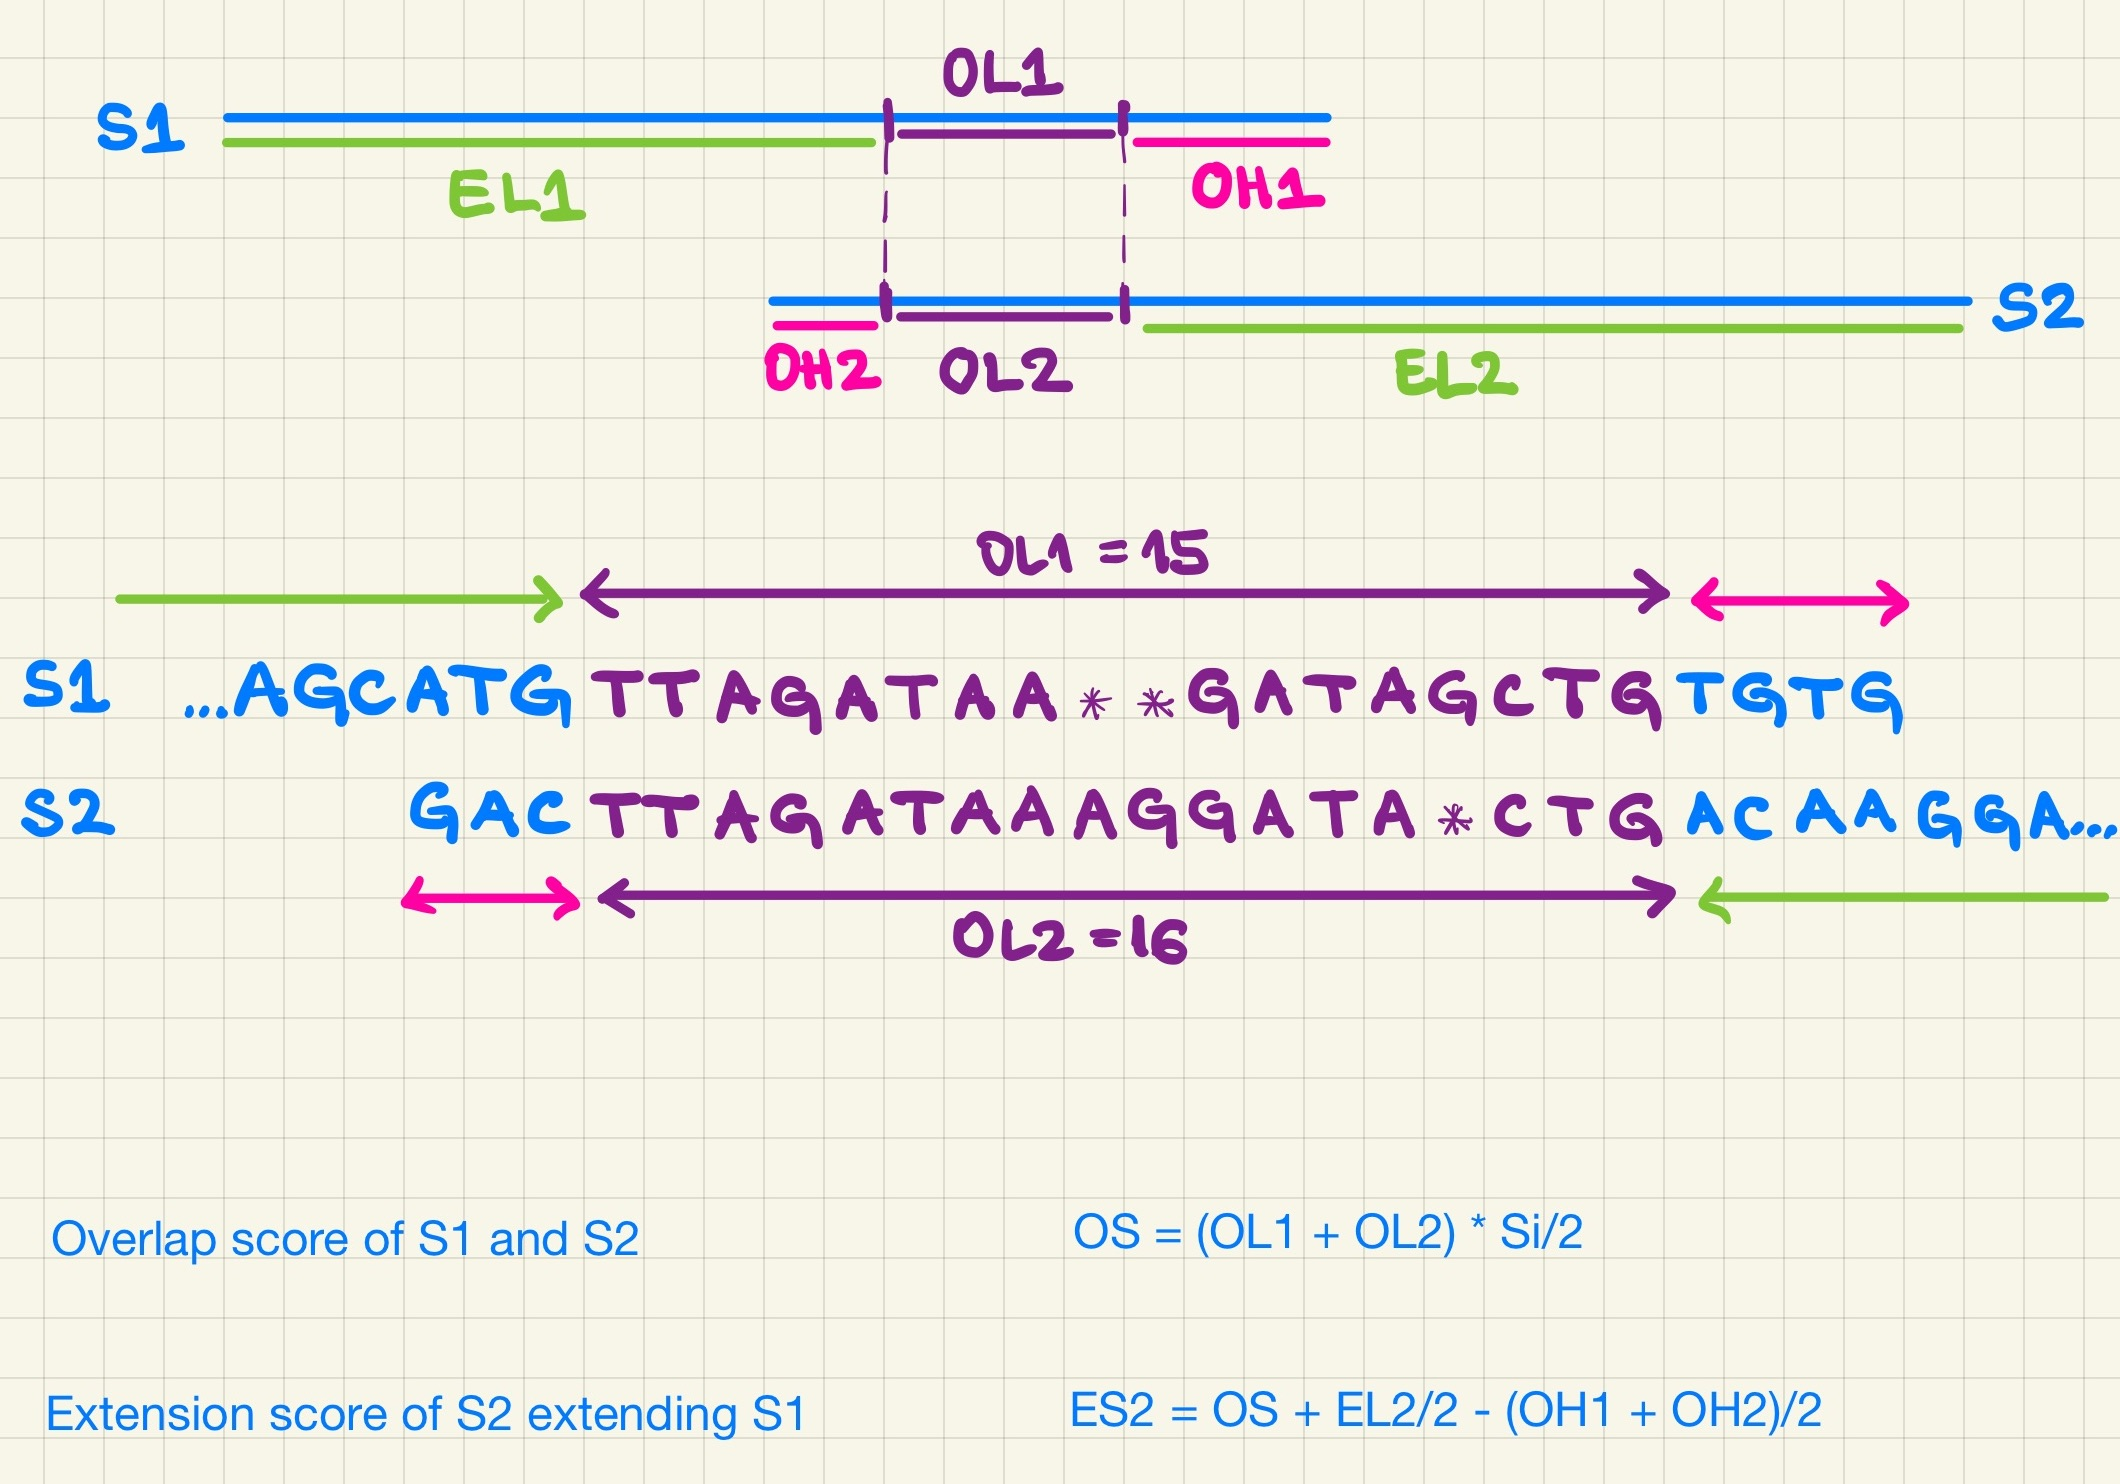
\includegraphics[width=\textwidth]{scores.jpg}
  \caption{Postupak računanja vrijednosti preklapanja i nadovezivanja}
  \label{fig:scores}
\end{figure}

\end{itemize}
\end{flushleft}

\newpage
\section{Koraci algoritma}
\subsubsection{Korak 1: Konstrukcija grafa preklapanja}
Konstruirati graf preklapanja koji će povezati fragmentirane contige i očitanja

\begin{figure}[H]
  \centering
  \includegraphics[width=\textwidth]{graph.png}
  \caption{Primjer grafa preklapanja}
  \label{fig:graph}
\end{figure}

\subsubsection{Korak 2: Identifikacija usidrenih čvorova}
Identificirati usidrene čvorove u grafu preklapanja.

\subsubsection{Korak 3: Pronalaženje optimalnih staza}
Pronaći optimalne staze iz svakog usidrenog čvora do mogućih završnih usidrenih čvorova. Ove staze određuju kako će se fragmentirani contigi povezivati međusobno.
\newline
(ctg1 -> read1-> read5 -> ctg2)

\subsubsection{Korak 4: Povezivanje contiga}
Na temelju optimalnih staza, povezati fragmentirane contige u cijeli genom. Koristititi informacije o preklapanju i veze između contig-a i očitanja i očitanja i očitanja kako bismo dobili ispravno generirani genom.

\chapter{Rezultati testiranja}
Analiziramo vrijeme izvođenja algoritma i količinu zauzete memorije.
\section{Vrijeme izvođenja}
Konstruiranje grafa na temelju:
\begin{itemize}
    \item[•]{overlap score: 1.415 milliseconds}
    \item[•]{extension score: 1.721 milliseconds}
    \item[•]{MonteCarlo metoda: 1.515 milliseconds}
\end{itemize}

\section{Količina zauzete memorije}
Konstruiranje grafa na temelju:
\begin{itemize}
    \item[•]{overlap score: 475.621 MB}
    \item[•]{extension score: 478.988 MB}
    \item[•]{MonteCarlo metoda: 476.492 MB}
\end{itemize}

\chapter{Zaključak}
Napravili smo algoritam za poboljšanje djelomično sastavljenog genoma dugim očitanjima. Korištenjem grafa preklapanja i traženjem optimalnih staza, uspjeli smo povezati fragmentirane contige u cijeli genom. Naš algoritam koristi preklapanja dobivena alatom Minimap2 kao ulazne podatke i generira poboljšani skup sastavljenih contiga u FASTA formatu kao izlaz.
\newline
\\Testiranjem algoritma, proučavali smo vrijeme izvođenja i količinu zauzete memorije. Rezultati su pokazali da je naš algoritam učinkovit i može se primijeniti na velike skupove podataka s minimalnim resursnim zahtjevima.
\newline
\\Zaključno, naš algoritam za poboljšanje djelomično sastavljenog genoma dugim očitanjima pokazao se kao koristan alat u području bioinformatike. Daljnjom primjenom i nadogradnjom ovog algoritma možemo pridonijeti rješavanju problema sastavljanja genoma i razumijevanju složenih genomskih struktura.

\bibliography{literatura}
\bibliographystyle{fer}

\end{document}
